%        File: !comp!expand("%:p:t")!comp!
%     Created: !comp!strftime("%a %b %d %I:00 %p %Y ").substitute(strftime('%Z'), '\<\(\w\)\(\w*\)\>\(\W\|$\)', '\1', 'g')!comp!
% Last Change: !comp!strftime("%a %b %d %I:00 %p %Y ").substitute(strftime('%Z'), '\<\(\w\)\(\w*\)\>\(\W\|$\)', '\1', 'g')!comp!
%
\documentclass[a4paper]{article}
\usepackage[catalan]{babel}
\usepackage[utf8]{inputenc}
\usepackage[obeyspaces]{url}
\usepackage{comment}
\usepackage{hyperref}
\usepackage[pdftex]{graphicx}
\begin{document}
\title{Instal·lació de Debian en un RAID1}
\maketitle

\begin{comment}
oddsidemargin \the\oddsidemargin \newline
textwidth \the\textwidth \newline
marginparsep \the\marginparsep \newline
marginparwidth \the\marginparwidth \newline
hoffset \the\hoffset \newline
paperwidth \the\paperwidth 
\end{comment}

\section{Què tenim a l'inici}
Dos discos iguals amb els quals volem muntar el raid1 sobre la instal·lació del sistema operatiu Debian 8.
\section{Particionat}
\paragraph{1. Escollim el mètode manual per particionar\\}
\paragraph{2. Fiquem una taula de particions buïda en cadascún dels dos discos\\}
\paragraph{3. Particionem \\ }
Particionem cadascun dels discos indicant que les particions que creem són volums d'un raid.\\

\scalebox{.5}{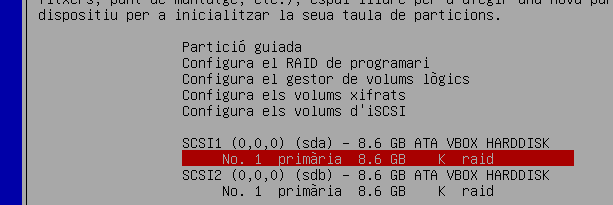
\includegraphics{3_marquem_particions.png}} \\
\scalebox{.5}{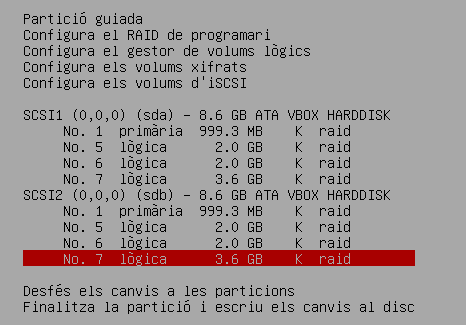
\includegraphics{3_final_marcat_particions.png}} \\
\paragraph{4. Configurem el RAID \\}
Escrivim els canvis fets al punt 3 i comencem a crear els dispositius MD associant per cada MD una partició amb la seva partició mirall.\\
\scalebox{.5}{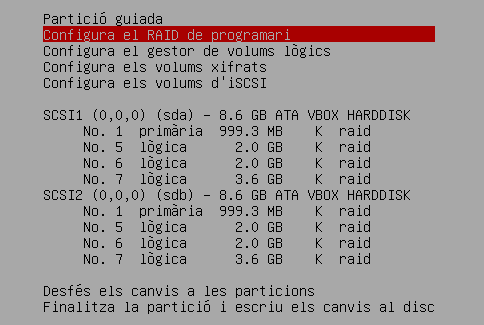
\includegraphics{4_configure_raid.png}} \\
\scalebox{.5}{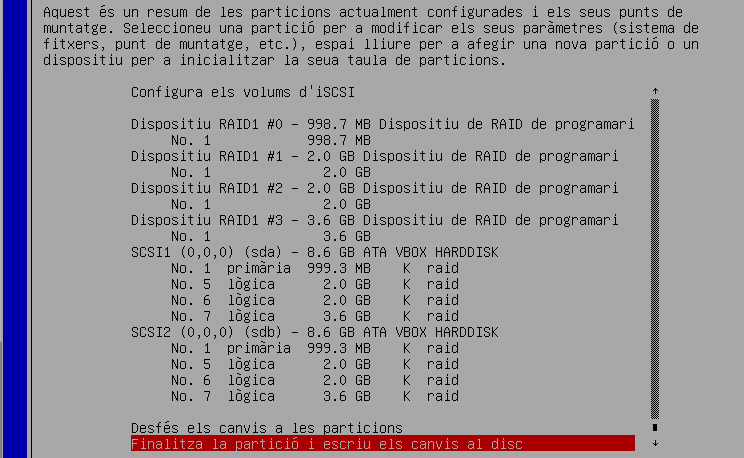
\includegraphics{4_fi_configure_raid.png}} \\
\paragraph{5. Muntem els dispositius MD \\}
\scalebox{.5}{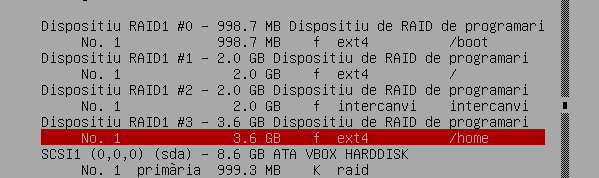
\includegraphics{5_Muntem_particions.png}} \\
\paragraph{6. Instal·lació del grub}
Durant el proc\'es d'instal·lació del Debian instal·lem el grub en el disc dur principal. Despr\'es, un cop reiniciada la màquina, instal·lem manualment el grub en l'altre disc.
\begin{verbatim}
# grub-install /dev/sdb
\end{verbatim}
\section{Test i monitorització}
\paragraph{fitxer /proc/mdstat\\}
Aquest \'es un exemple en el que fem un raid 1 de les particions /, /boot, /swap i /home i en el que l'estat \'es correcte:
\begin{verbatim}
# cat /proc/mdstat 
Personalities : [raid1] 
md3 : active raid1 sda7[0] sdb7[1]
      3502080 blocks super 1.2 [2/2] [UU]
			      
md2 : active (auto-read-only) raid1 sda6[0] sdb6[1]
			1950720 blocks super 1.2 [2/2] [UU]
						      
md1 : active raid1 sda5[0] sdb5[1]
      1950720 blocks super 1.2 [2/2] [UU]
									      
md0 : active raid1 sda1[0] sdb1[1]
 			975296 blocks super 1.2 [2/2] [UU]
												      
unused devices: <none>
\end{verbatim}
El fitxer /proc/mdstat et dona una foto de com estan els dispositius raid. Mirem un altre exemple:
\begin{verbatim}
md_d0 : active raid5 sde1[0] sdf1[4] sdb1[5] sdd1[2] sdc1[1]
\end{verbatim}
El que vol dir \'es que \verb+md_d0+ \'es un raid 5 format per /dev/sde1, el qual \'es el dispositiu 0, el sdf1 que \'es el 4, etc. Fixeu-vos que falta el 3, això \'es perque el dispositiu 3 ha fallat i ha sigut canviat per el 5. Tots els dispusitius que tinguin un nombre m\'es gran que el que marca el raid - 1 són inicialment, \textit{spares}. Un altre exemple: 
\begin{verbatim}
[==>.............]  recovery = 12.6% (37043392/292945152) finish=127.5min speed=33440K/sec
\end{verbatim}
Això \'es una mostra de proc\'es de recuperació d'un raid. Teniu m\'es apunts en \cite{PROCMDSTAT}.
\paragraph{Comanda mdadm \\}
\begin{verbatim}
mdadm --detail /dev/mdx
\end{verbatim}
Aquesta comanda mostrarà els discos o particions que han fallat i els que hi han de reposició.
\paragraph{Simulant la fallida \\}
Ara simularem amb la comanda \verb+mdadm+ la fallida del disc \verb+/dev/sda+, mirarem a on ens donen els avisos de fallida el sistema i despr\'es iniciarem el sistema per veure que ho fa perfectament des del disc 2 (d'això últim no n'hi han imatges).\\
\scalebox{.5}{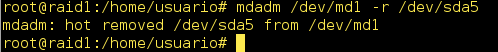
\includegraphics{simulant_fallida.png}} \\
\scalebox{.5}{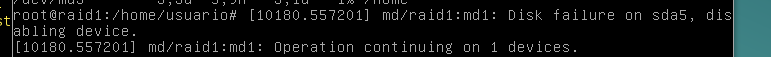
\includegraphics{fallida_logs_1.png}} \\
\scalebox{.5}{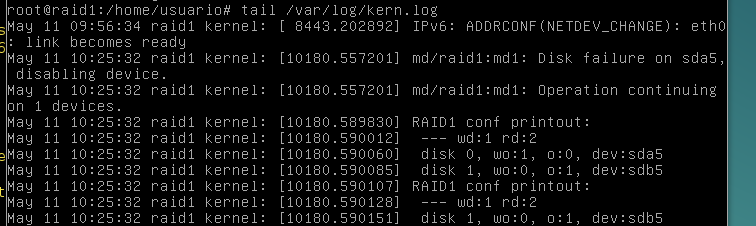
\includegraphics{fallida_logs_2.png}} \\
\scalebox{.5}{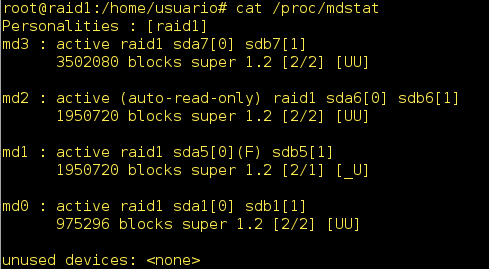
\includegraphics{fallida_logs_3.png}} \\
\scalebox{.5}{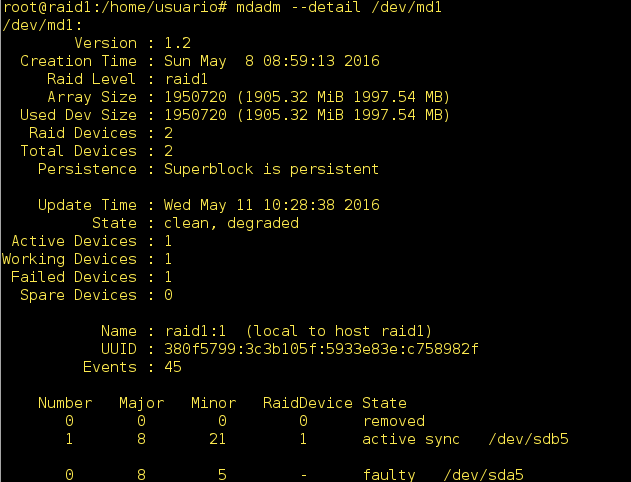
\includegraphics{fallida_logs_4.png}} \\
\section{Sobre aquest document}
\textbf{Copyright}\copyright\ \textbf{\the\year\ Juan Aguilera}.\\
Permission is granted to copy, distribute and/or modify this document under the terms of the GNU Free Documentation License, Version 1.3 or any later version published by the Free Software Foundation;\\
with no Invariant Sections, no Front-Cover Texts, and no Back-Cover Texts.\\
A copy of the license is included in the section entitled \href{http://www.gnu.org/licenses/fdl.html}{``GNU Free Documentation License``}.

\begin{thebibliography}{99}
		% Exemple url: \bibitem{Debian} \url{https://wiki.debian.org/es}%
		\bibitem{INSTALL} \url{https://blog.sleeplessbeastie.eu/2013/10/04/how-to-configure-software-raid1-during-installation-process/}
		\bibitem{PROCMDSTAT} \url{https://raid.wiki.kernel.org/index.php/Mdstat}
		\bibitem{TEST} \url{https://raid.wiki.kernel.org/index.php/Detecting,_querying_and_testing}
\end{thebibliography}
\end{document}
